\documentclass[11pt,tikz,border=6mm]{standalone}
\usepackage[T1]{fontenc}
\usepackage{lmodern}
\usepackage{tikz}
\usetikzlibrary{arrows.meta,positioning,calc,shapes.multipart}

\definecolor{umlInk}{HTML}{263445}
\definecolor{umlAccent}{HTML}{285B80}
\definecolor{umlHeader}{HTML}{E9F1F6}
\definecolor{umlNote}{HTML}{F7F8FA}

% Copy this style block into each diagram; change shared values here.
\tikzset{
  uml/base/.style={draw=umlInk,text=umlInk,line width=0.65pt,
    font=\sffamily\small,inner xsep=5pt,inner ysep=5pt,outer sep=0.4pt},
  uml/class/.style={uml/base,rectangle split,rectangle split parts=3,
    rectangle split ignore empty parts=false,
    rectangle split part fill={umlHeader,white,white},
    rectangle split part align={center,left,left},
    text width=42mm,align=center},
  uml/component/.style={uml/base,rectangle,fill=umlHeader,text width=42mm,align=center},
  uml/note/.style={uml/base,rectangle,fill=umlNote,text width=83mm,align=left},
  uml/label/.style={font=\sffamily\footnotesize,text=umlInk,
    inner sep=1.5pt,fill=white},
  uml/edge/.style={draw=umlInk,line width=0.65pt},
  uml/association/.style={uml/edge},
  uml/dependency/.style={uml/edge,dashed,-{Straight Barb[length=3mm,width=2mm]}},
  uml/generalization/.style={uml/edge,-{Triangle[open,length=3.2mm,width=3.2mm]}},
  uml/realization/.style={uml/generalization,dashed},
  uml/aggregation/.style={uml/edge,{Diamond[open,length=3.4mm,width=2.6mm]}-},
  uml/composition/.style={uml/edge,{Diamond[fill=umlInk,length=3.4mm,width=2.6mm]}-},
  uml/note-link/.style={uml/edge,densely dashed},
  uml/lifeline/.style={uml/edge,densely dashed},
  uml/call/.style={uml/edge,-{Triangle[length=3mm,width=2.2mm]}},
  uml/async/.style={uml/edge,-{Straight Barb[length=3mm,width=2mm]}},
  uml/reply/.style={uml/edge,dashed,-{Straight Barb[length=3mm,width=2mm]}}
}

\begin{document}
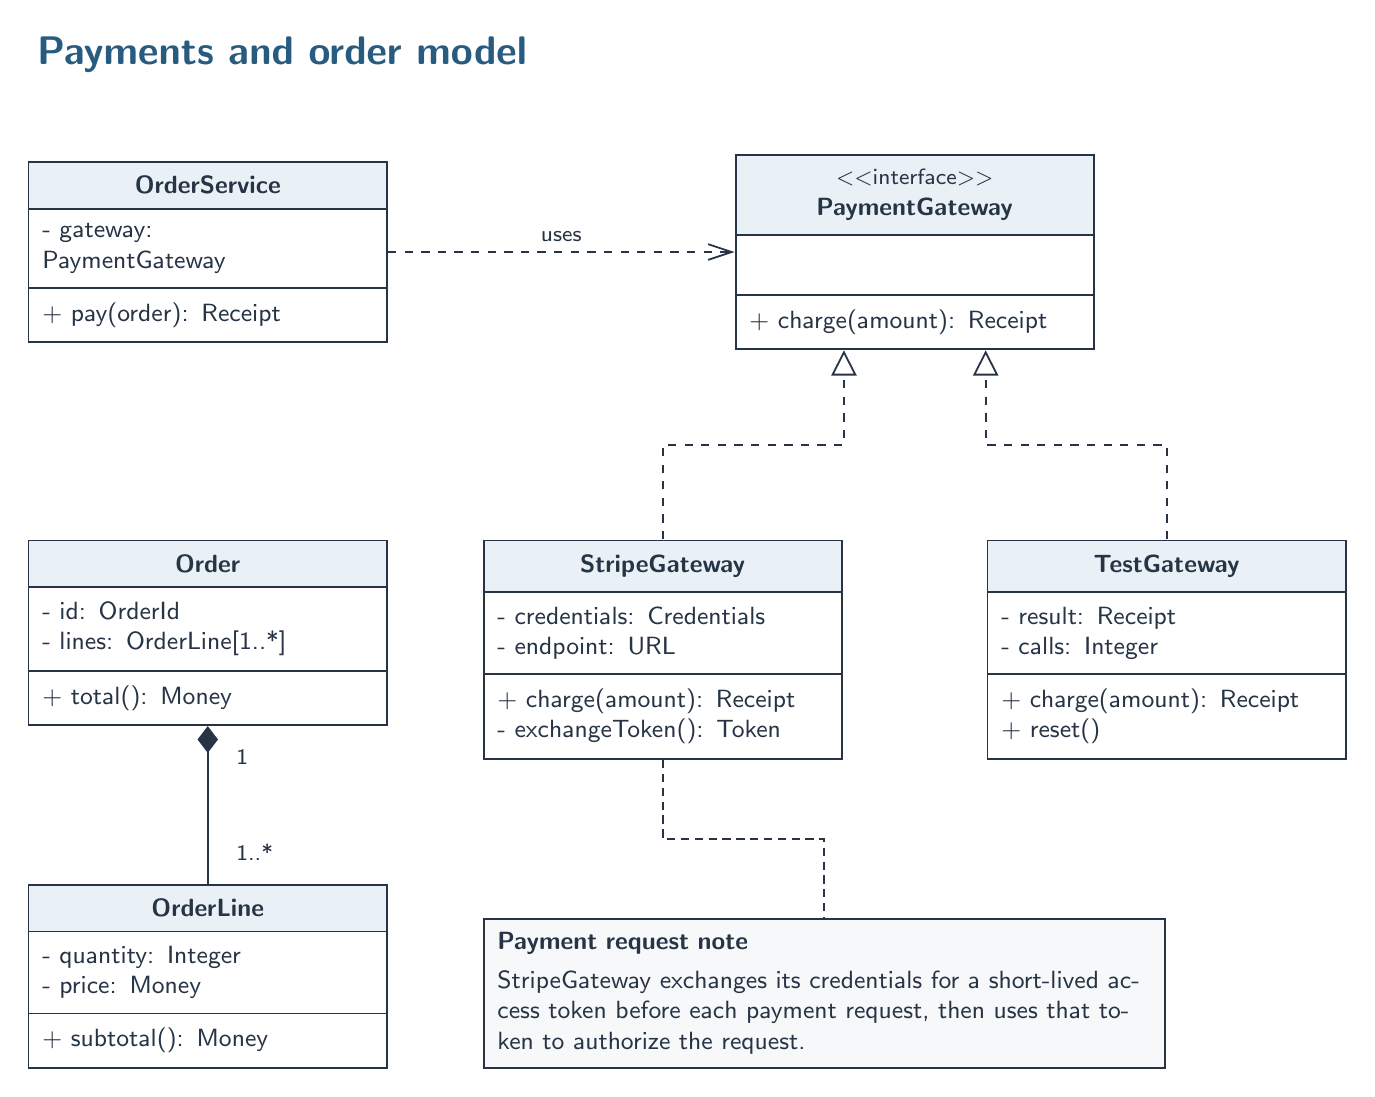
\begin{tikzpicture}
\node[uml/class] (gateway) {
  {\footnotesize\normalfont\sffamily\textless\textless interface\textgreater\textgreater}\\
  \textbf{PaymentGateway}
  \nodepart[align=left]{two}\strut
  \nodepart[align=left]{three}
  + charge(amount): Receipt
};
\node[uml/class,left=44mm of gateway] (service) {
  \textbf{OrderService}
  \nodepart[align=left]{two}
  - gateway:\\PaymentGateway
  \nodepart[align=left]{three}
  + pay(order): Receipt
};

% The implementation row has equal widths and a clear routing corridor above.
\coordinate (implementation-row) at ([yshift=-24mm]gateway.south);
\node[uml/class,anchor=north] (stripe)
  at ([xshift=-32mm]implementation-row) {
  \textbf{StripeGateway}
  \nodepart[align=left]{two}
  - credentials: Credentials\\
  - endpoint: URL
  \nodepart[align=left]{three}
  + charge(amount): Receipt\\
  - exchangeToken(): Token
};
\node[uml/class,anchor=north] (test)
  at ([xshift=32mm]implementation-row) {
  \textbf{TestGateway}
  \nodepart[align=left]{two}
  - result: Receipt\\
  - calls: Integer
  \nodepart[align=left]{three}
  + charge(amount): Receipt\\
  + reset()
};

\node[uml/class,anchor=north] (order)
  at (service.center |- implementation-row) {
  \textbf{Order}
  \nodepart[align=left]{two}
  - id: OrderId\\
  - lines: OrderLine[1..*]
  \nodepart[align=left]{three}
  + total(): Money
};
\node[uml/class,below=20mm of order] (line) {
  \textbf{OrderLine}
  \nodepart[align=left]{two}
  - quantity: Integer\\
  - price: Money
  \nodepart[align=left]{three}
  + subtotal(): Money
};
\node[uml/note,anchor=north west] (token-note)
  at ([yshift=-20mm]stripe.south west) {
  \textbf{Payment request note}\\[3pt]
  StripeGateway exchanges its credentials for a short-lived access token
  before each payment request, then uses that token to authorize the request.
};

\draw[uml/dependency] (service.east) --
  node[uml/label,midway,above=2pt] (uses-label) {uses} (gateway.west);

\coordinate (left-port) at ([xshift=-9mm]gateway.south);
\coordinate (right-port) at ([xshift=9mm]gateway.south);
\coordinate (left-lane) at ([yshift=12mm]stripe.north);
\coordinate (right-lane) at ([yshift=12mm]test.north);
\draw[uml/realization]
  (stripe.north) -- (left-lane) -- (left-port |- left-lane) -- (left-port);
\draw[uml/realization]
  (test.north) -- (right-lane) -- (right-port |- right-lane) -- (right-port);

% Start at the whole: the composition diamond belongs beside Order.
\draw[uml/composition] (order.south) --
  node[uml/label,pos=.20,right=3mm] (owner-count) {1}
  node[uml/label,pos=.80,right=3mm] (line-count) {1..*}
  (line.north);

\draw[uml/note-link]
  (stripe.south) -- ++(0,-10mm) -| (token-note.north);

\node[font=\sffamily\Large\bfseries,text=umlAccent,anchor=south west]
  at ([yshift=10mm]service.north west) {Payments and order model};
\end{tikzpicture}
\end{document}
